\documentclass[a4paper,addpoints]{exam}

\usepackage{commath}
\usepackage[framemethod=tikz]{mdframed}
\usepackage{siunitx}

% russian integral
\usepackage{scalerel}
\DeclareMathOperator*{\rint}{\scalerel*{\rotatebox{17}{$\!\int\!$}}{\int}}

\qformat{\textbf{\large{Question \thequestion}}\hfill}
\pointsinrightmargin

\begin{document}

\begin{coverpages}

\begin{center}
  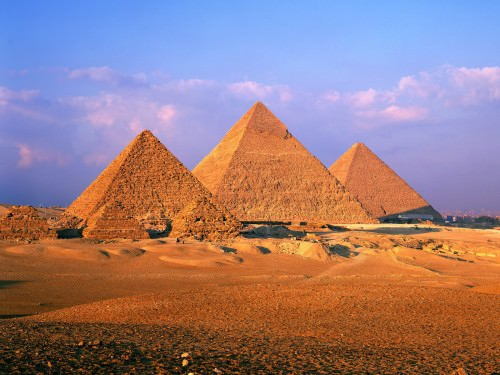
\includegraphics[width=0.6\textwidth]{exam-cover-07}

  \vspace{5mm}

  \textbf{\Huge{Scholarship Calculus}}

\end{center}

\vspace{5mm}

\noindent
\large{There are five questions, worth a total of \numpoints\ marks.\\
       Attempt ALL questions, showing all working.\\
       Choose ONE option ONLY from 2(b) and 2(c).\\
       Read questions carefully before attempting them.\\
       Marks are available for partial answers.\\
       The amount of time expected to be spent per question may not necessarily correlate ``nicely'' to the number of marks.\\
       Diagrams may be used to support answers.\\
       Candidates who do not provide diagrams for some questions may be disadvantaged.\\
       Some marks are given for clarity and neatness of solutions or proofs.}
\vspace{2mm}

\begin{tabular}{ll}
  \textbf{Time Allowed:}& Three Hours\\
  \textbf{Scholarship:}& 45 marks\\
  \textbf{Outstanding:}& 65 marks
\end{tabular}

\vfill

\begin{center}
  \gradetable[h][questions]
  \vspace{5mm}

  \textbf{Available Grades:} \quad\textit{No Scholarship}\qquad\textit{Scholarship}\qquad\textit{Outstanding}
\end{center}

\end{coverpages}

\begin{questions}
  \question
    \begin{parts}
      \part[5] Consider the sequence of functions
            \begin{displaymath}
              f_n(x) = nx(1 - x^2)^n \qquad\text{($0 \leq x \leq 1 $, $ n = 1, 2, 3, ... $)}.
            \end{displaymath}
            Show that
            \begin{displaymath}
              \lim_{n \to \infty} \rint^1_0 f_n(x) \dif{x} \neq \rint^1_0 \lim_{n \to \infty} f_n(x) \dif{x}.
            \end{displaymath}
      \part[5] Compute the following definite integral.
            \begin{displaymath}
              \rint^1_0 \sin^3 x \cos^4 x + \sin^4 x \cos^3 x \dif{x}.
            \end{displaymath}
      \part[5] Suppose that $ f $ is a function satisfying
            \begin{displaymath}
              \begin{cases}
                \dfrac{f(x)}{2f'(x)} = 3(x^3 - 2x^2 - x + 2),\\
                f(3) = 1.
              \end{cases}
            \end{displaymath}
            Find $ f(x) $ explicitly. You need only calculate any constants of integration to three decimal places.
    \end{parts}
  \question
    \begin{parts}
      \part[10] Consider the cubic equation $ p(x) = x^3 + px + q $ (where $ p $ and $ q $ are real).
        \begin{subparts}
          \subpart Let the three roots of $ p(x) $ be $ \alpha $, $ \beta $, and $ \gamma $. Show that
                   \begin{displaymath}
                     (\alpha - \beta)^2(\beta - \gamma)^2(\gamma - \alpha)^2 = -4p^3 - 27q^2.
                   \end{displaymath}
          \subpart Find the nature of the roots of $ p(x) $ in the cases where $ -4p^3 - 27q^2 $ is greater than, less than, or equal to zero.
        \end{subparts}
      \fullwidth{\textbf{Answer ONE of (b) and (c).}}
      \noaddpoints
      \part[5] Find a formula for $ \binom{n - 1}{k} - \binom{n - 1}{k - 1} $ in terms of $ \binom{n}{k} $.
      \addpoints
      \part[5] Minimise $ F(x) = x^3 + y^4 + z^5 $ with respect to the variables $ x $, $ y $, and $ z $ subject to:
            \begin{gather*}
              x + y + z \geq 1\\
              x - y + z \leq 2\\
              z \geq 2\\
              0.75x - 5.87y - 5.78z \geq -31.74.
            \end{gather*}
            \textit{A graph of these planes is provided on the final page of this examination.}
    \end{parts}
  \question
    \begin{parts}
      \part[5] Find $ \od{}{x} (\sec x)(\sec^{-1} x) $ in terms of $ x $ only.
      \part[5] Consider a circle of radius $ r $ that is rolling around the inside of a circle of radius $ R $ ($ R > r $). Let $ p = (x,y) $ be
            the point on the inner circle that is initially touching the outer circle. Show that
            \begin{align*}
              x &= (R - r) \cos \theta + \cos\left(\frac{R - r}{r} \theta\right),\\
              y &= (R - r) \sin \theta - \sin\left(\frac{R - r}{r} \theta\right).
            \end{align*}
            \textit{A diagram is provided on the final page of this examination.}
      \part[5] The Steiner inellipse is the unique ellipse inscribed in a triangle and tangent to the midpoint of each side. Find the coordinates of the
            two focii of the Steiner inellipse inscribed in the triangle with vertices $ (1, 7) $, $ (7, 5) $, and $ (3, 1) $.
    \end{parts}

  \clearpage
  \question
    \begin{parts}
      \part[5]
        \begin{subparts}
          \subpart By differentiating $ f(x) g(x) $, show that
                   \begin{displaymath}
                     \rint f'(x) g(x) \dif{x} = f(x) g(x) - \rint f(x) g'(x) \dif{x}.
                   \end{displaymath}
          \subpart Find an antiderivative of
                   \begin{displaymath}
                     \frac{\sqrt{4x^2 - 9}}{x^2}.
                   \end{displaymath}
        \end{subparts}
      \part[5] Discuss the significance of the fundamental theorem of calculus. You should write approximately half a page.
      \part[5] An \textbf{automorphism} is a function $ f $ such that $ f(a + b) = f(a) + f(b) $ and $ f(ab) = f(a) f(b) $ for \emph{all} real
            numbers $ a $ and $ b $. Show that
            \begin{displaymath}
              f(x) = \begin{cases}
                       1 & \text{if $ x $ is even}\\
                       -1 & \text{if $ x $ is odd}
                     \end{cases}
            \end{displaymath}
            is an automorphism.
    \end{parts}
  \question
    You may use the following theorem in answering this question. \textbf{Do not attempt to prove this theorem.}

    \begin{mdframed}
      \textbf{Mean Value Theorem}\\
      Let $ a $ and $ b $ be real numbers such that $ a < b $, and let $ f $ be a function satisfying two hypotheses:
      \begin{enumerate}
        \item $ f $ is continuous at all $ x $ such that $ a < x < b $.
        \item $ f $ is differentiable at all $ x $ such that $ a \leq x \leq b $.
      \end{enumerate}
      Then there exists some number $ c $ such that
      \begin{displaymath}
        f'(c) = \frac{f(b) - f(a)}{b - a}.
      \end{displaymath}
    \end{mdframed}

    \begin{parts}
      \part[5] Verify that the function $ f $ defined by
            \begin{displaymath}
              f(x) = \frac{x}{x + 2}
            \end{displaymath}
            satisfies the hypotheses of the mean value theorem on the interval $ 1 < x < 4 $. Find all points $ c $ that satisfy the conclusion
            of the mean value theorem.
      \part[5] A point $ a $ is called a \textbf{fixed point} of a function $ f $ if $ f(a) = a $. Suppose that $ f'(x) \neq 1 $ for all real numbers $ x $;
            show that $ f $ has at most one fixed point.
      \part[5] Find a function $ f $ such that $ f'(-1) = \frac{1}{2} $, $ f'(0) = 0 $, and $ f''(x) > 0 $ for all $ x $, or prove that such a function
            cannot exist.
    \end{parts}
\end{questions}

\vspace*{\fill}
\textbf{Figures provided overleaf.}
\clearpage

\section*{Useful Figures}

\begin{center}
  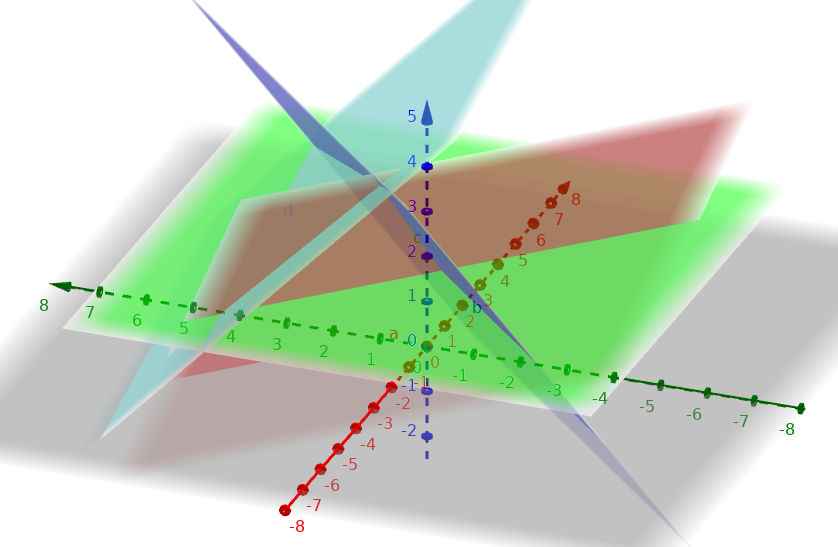
\includegraphics[width=\textwidth]{nasty-inequalities}\\
  \textit{Question 2(c)}

  \vspace*{2cm}

  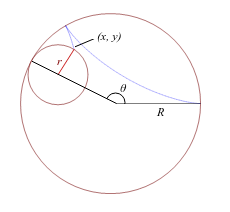
\includegraphics[width=0.4\textwidth]{hypo}\\
  \textit{Question 3(b)}
\end{center}

\end{document}
